\documentclass[UTF8]{ctexart}
\usepackage{geometry, CJKutf8,tikz}
\geometry{margin=1.5cm, vmargin={0pt,1cm}}
\setlength{\topmargin}{-1cm}
\setlength{\paperheight}{29.7cm}
\setlength{\textheight}{25.3cm}

% useful packages.
\usepackage{amsfonts}
\usepackage{amsmath}
\usepackage{amssymb}
\usepackage{amsthm}
\usepackage{enumerate}
\usepackage{graphicx}
\usepackage{multicol}
\usepackage{fancyhdr}
\usepackage{layout}
\usepackage{listings}
\usepackage{float, caption}

\lstset{
    basicstyle=\ttfamily, basewidth=0.5em
}

% some common command
\newcommand{\dif}{\mathrm{d}}
\newcommand{\avg}[1]{\left\langle #1 \right\rangle}
\newcommand{\difFrac}[2]{\frac{\dif #1}{\dif #2}}
\newcommand{\pdfFrac}[2]{\frac{\partial #1}{\partial #2}}
\newcommand{\OFL}{\mathrm{OFL}}
\newcommand{\UFL}{\mathrm{UFL}}
\newcommand{\fl}{\mathrm{fl}}
\newcommand{\op}{\odot}
\newcommand{\Eabs}{E_{\mathrm{abs}}}
\newcommand{\Erel}{E_{\mathrm{rel}}}

\begin{document}

\pagestyle{fancy}
\fancyhead{}
\lhead{姓名: 邓东宁}
\chead{数据结构与算法作业5}
\rhead{学号: 3230101177}
\cfoot{Oct.31th, 2024}
\section{函数remove()改进思路}
原本的函数虽然可读性强,但涉及元素复制(效率不可控),且重复搜索,故针对这些问题进行改进。\\
改进的主要想法是先找到待删除的节点,但查找方法和原本的不一样,我在查找时保持了对当前迭代节点的父节点parentNode的追踪,确保后续删除节点后,我们可利用手持的父节点正确地重新连接子树(当然parentNode在待删除节点就是根节点时为空,此时无需考虑重新连接问题,这点我也考虑进了实际代码中)。找到待删除节点后,藉助新增函数detachMin()找到其右子树的最小节点,返回的同时将其从原本的位置正确地摘除(不是删除),接着用其正确地替换掉待删除节点,最后从内存中删除待删除节点。\\
\textbf{以下是找到待删除节点后具体的讨论内容:}
\begin{itemize}

  \item \textbf{如果待删除节点无右子树},则直接让其左子树连接到其父节点上
  \item \textbf{如果待删除节点有右子树,且右子树第一个节点就是最小节点}(即第一个节点无左子树),则让该节点继承待删除节点的左子树,然后连接到待删除节点的父节点上
  \item \textbf{如果待删除节点有右子树,且右子树第一个节点不是最小节点}(即第一个节点有左子树),则让该节点继承待删除节点的左、右子树,然后连接到待删除节点的父节点上
\end{itemize}
\section{测试程序的设计思路}

测试用例按原本的来:\\\\
\begin{tikzpicture}[level/.style={sibling distance=75pt/#1, level distance=36pt},
                    every node/.style={align=center, inner sep=0, minimum size=20pt}]
\node [draw, circle]
    {10}
    child {node[draw, circle] {5}
        child {node[draw, circle] {3}}
        child {node[draw, circle] {7}}}
    child {node[draw, circle] {15}
        child {node[draw, circle] {12}}
        child {node[draw, circle] {18}}};
\end{tikzpicture}\\\\
测试事项:
\begin{itemize}
  \item 删除数据3,测试情况1中,删除非根节点的子情况:\\\\
\begin{tikzpicture}[level/.style={sibling distance=75pt/#1, level distance=36pt},
                    every node/.style={align=center, inner sep=0, minimum size=20pt}]
\node [draw, circle]
    {10}
    child {node[draw, circle] {5}
        child {node[draw, circle] {7}}}
    child {node[draw, circle] {15}
        child {node[draw, circle] {12}}
        child {node[draw, circle] {18}}};
\end{tikzpicture}\\
  \item 删除数据5,测试情况2中,删除非根节点的子情况:\\\\
\begin{tikzpicture}[level/.style={sibling distance=75pt/#1, level distance=36pt},
                    every node/.style={align=center, inner sep=0, minimum size=20pt}]
\node [draw, circle]
    {10}
    child {node[draw, circle] {7}}
    child {node[draw, circle] {15}
        child {node[draw, circle] {12}}
        child {node[draw, circle] {18}}};
\end{tikzpicture}\\
  \item 删除数据15,测试情况3中,删除非根节点的子情况:\\\\
\begin{tikzpicture}[level/.style={sibling distance=75pt/#1, level distance=36pt},
                    every node/.style={align=center, inner sep=0, minimum size=20pt}]
\node [draw, circle]
    {10}
    child {node[draw, circle] {7}}
    child {node[draw, circle] {12}
        child {node[draw, circle] {18}}};
\end{tikzpicture}\\
  \item 删除数据10,测试删除根节点的情况:\\\\
\begin{tikzpicture}[level/.style={sibling distance=75pt/#1, level distance=36pt},
                    every node/.style={align=center, inner sep=0, minimum size=20pt}]
\node [draw, circle]
    {12}
    child {node[draw, circle] {7}}
    child {node[draw, circle] {18}};
\end{tikzpicture}\\
\end{itemize}

\section{测试结果}
所有结果符合预期,未发现异常;未测试内存泄漏存在性,烦请助教检验

\section{遇到的挑战}
在测试时,我发现如果删除的是根节点,那么下次就无法输出了,让我百思不得其解。\\
后来我发现这是因为删除根节点的同时,连带删除了BST对象的根节点root属性,而printTree()是根据root来运作的,所以要记得将BST对象的root属性更新为替换上来的节点。\\\\
最近几次作业过程中,凡是涉及指针,我总是容易创造bug,并且花费了大量时间去debug,让我无不感慨C++真的是一门很精细的语言,必须要予以内存管理足够的顾虑。我以前先后学过Java和Python,这些语言都有自己一套管理内存的机制,不需要顾虑这些,但也让我错失了对内存的深入认知机会,好在现在学了C++,虽然难度陡增,但也收获良多!

\end{document}
